\section*{Task \#4: Dynamic SSE}
    \subsection*{Introduction}
    In the previous task we performed SSE on a static system, now we leave out the static hypothesis and move into the dynamic one.
    In the dynamic setting the martix A is no longer the identity matrix and in order to solve this problem we couldn't use least square or Gradient Descent (GD) algorithms due to their performances. Instead we run a single GD step at each $k$ instant, this algorithm has been called the Online Gradient Descent or \textbf{OGD} and is used to develop a sparse observer
    
    \subsection*{Algorithms}
    The algorithm of the sparse observer is the following:
    \\Given $y(k) = Gz(k)$ and $\hat{z}(k)$
    \begin{equation} \label{eq:OGD}
        \begin{aligned}
            &\hat{z}^+(k) = \hat{z}(k) - \tau G^T[G\hat{z}(k) - y(k)]\\
            &\hat{x}(k+1) = A\hat{x}^+(k)\\
            &\hat{a}(k+1) = \mathbb{S}_{\tau \lambda}[\hat{a}^+(k)]\\
            &\hat{y}(k) = G \hat{z}(k)\\
        \end{aligned}    
    \end{equation}   
    
    \subsection*{Results}
    Below are the results presented in the following structure:
    \begin{itemize}
        \item Image: the image is further divided into two parts. On the left side $(a)$, a specific case of the results obtained by the execution of the algorithm after T time instant is shown, while on the right side $(b)$, the final situation of the room is presented, providing a snapshot of the SSE result after T time instants.
        \item Table: a summary table that gives information on the results obtained by running the algorithm 100 times under the same conditions in terms of: targets,sensors under attack,execution time ($T_{max}$) and type of attack carried out. This table is useful to understand how the algorithm generally behaves.
    \end{itemize}
\noindent
    The convergence of the attack $a$ and state $x$ are understood as a match between the support of the actual vector and the estimated vector. For the observer insted the convergence time is understood as intersection between the convergence of the two previous vector.
    \subsubsection*{Main task: unaware attack}
    Using $\Lambda = [10,...10,20..20]$, a time simulation of 50 and matrices $A,D,Y$ provided by the file $tracking\_moving\_targets.mat$ we obtain that in general the sparse observer converge in 34 time instants and in particular the positions of the targets are correctly estimated only after 23 time istants.
    
    \begin{figure}[!ht]   
        \vspace{-1cm}
        \centering 
        \subfigure[Convergence]
        {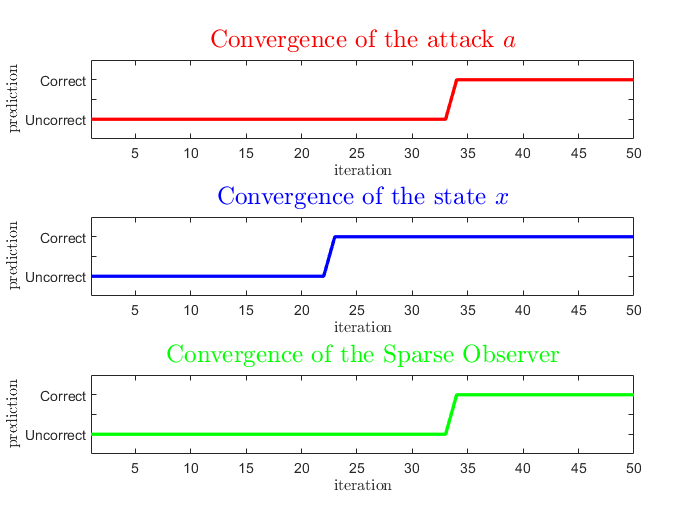
\includegraphics[scale=0.3]{img/unaware_2.png}}
        \subfigure[Room]
        {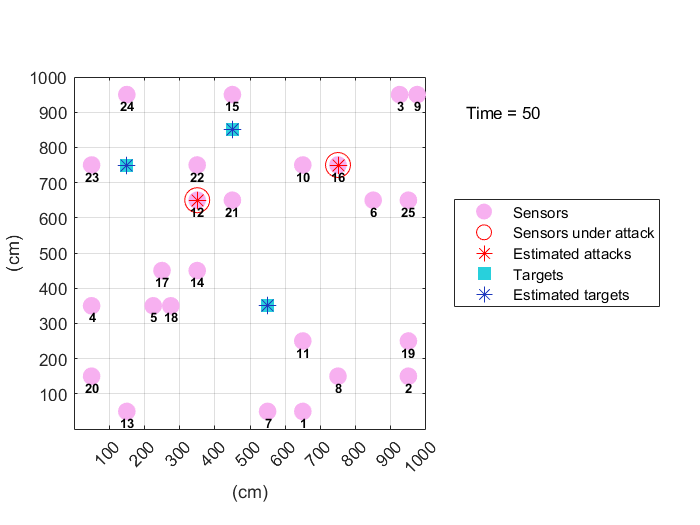
\includegraphics[scale=0.3]{img/unaware_1.png}}
        \caption{Unawere: Three targets and two sensors under attack}
        \label{fig:unaware_1}
    \end{figure}
    
    \noindent
    In this case the table was not reported because it would not add any additional information since the matrices used are always the same. In fact even running the algorithm 100 times we always get observer convergence with convergence times of the attack estimate of 34 time instants and 23 for the state

    
    \newpage
    \subsubsection*{1\# optional task: aware time-varying attack}
    For this first optional task, the A and D matrices are always the same while the Y matrix was computed starting from randomly generated initial conditions. At each time instant $k$ an attack equal to half the previous value of the output is injected on the actual output ($a(k)= \frac{1}{2}y(k-1) \forall k=1..50$). 
    \begin{figure}[h]   
        \vspace{-1cm}
        \centering 
        \subfigure[Convergence]
        {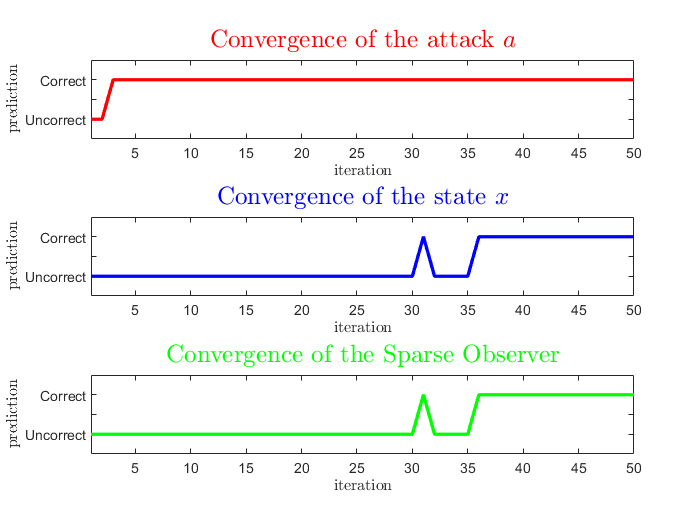
\includegraphics[scale=0.3]{img/aware_2a_3x_2.png}}
        \subfigure[Room]
        {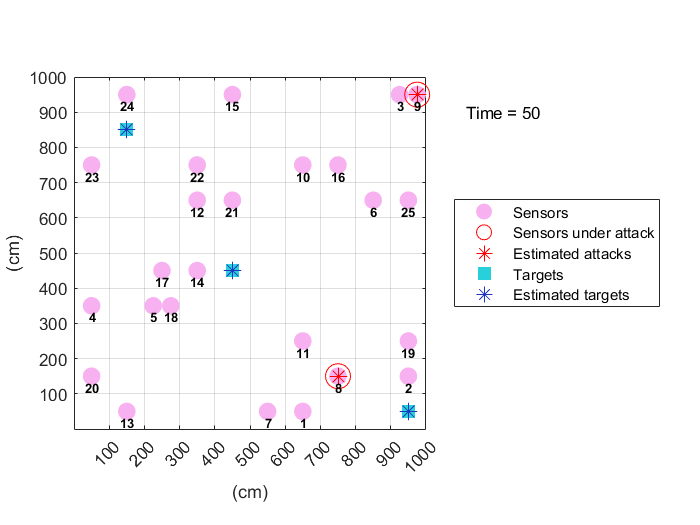
\includegraphics[scale=0.3]{img/aware_2a_3x_1.png}}
        \caption{Aware: Three targets and two sensors under attack}
        \label{fig:aware_2}
    \end{figure}
    
\noindent
As can be seen, in general, the sensors under attack are always correctly identified. However, regarding the position of the targets, only in 87\% of the cases, after 50 instant of time, a correct estimate is achieved.
    
\begin{table}[h!]
\centering
\begin{tabular}{|c|c|c|}
\hline
\multirow{2}{*}{\textbf{For 100 iterations}} & \multicolumn{1}{|c|}{\textbf{attack $a$}} & \multicolumn{1}{|c|}{\textbf{state $x$}} \\
\cline{2-3}
 & \textbf{1-50} & \textbf{1-50}\\
\hline
\textbf{\% convergence} &98\% &89\%  \\
\hline
\textbf{Mean time of convergene} &4.29 &30.46 \\
\hline
\textbf{Minimum time of convergence} &2 &10  \\
\hline
\textbf{Maximum time of convergence} &13 &50 \\
\hline
\textbf{Temporay loss of tracking} &2\% &58\%  \\
\hline
\end{tabular}
\caption{Summary table showing some statistics on $a$ and $x$}
\label{table:4}
\end{table}
            
    \subsubsection*{2\# changing sensors under attack}
For the second task, an additional complication was introduced by changing the sensors under attack every 25 instant of time. In the graph shown in the figure, it can be seen that, in general, this change of sensors under attack causes problems in tracking the targets, temporarily shifting the state prediction from correct to incorrect. In most cases, by the end of the 50 instants of time, the state is still correctly recovered.
\begin{figure}[h]   
    \vspace{-1cm}
    \centering 
    \subfigure[Convergence]
    {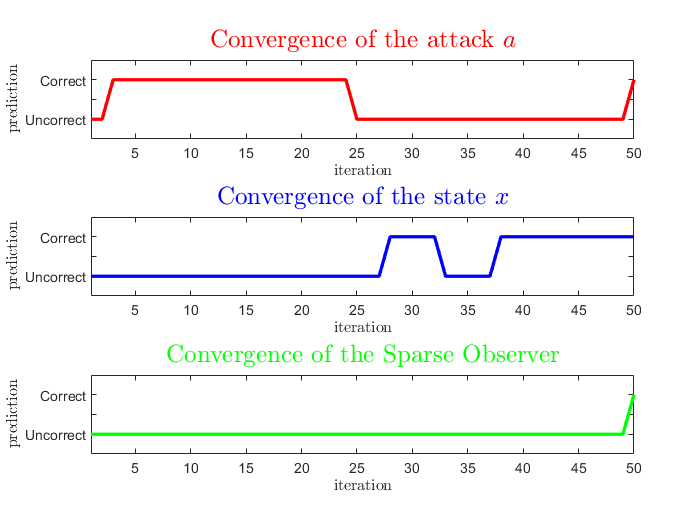
\includegraphics[scale=0.3]{img/aware_2a_3x_cs_2.png}}
    \subfigure[Room]
    {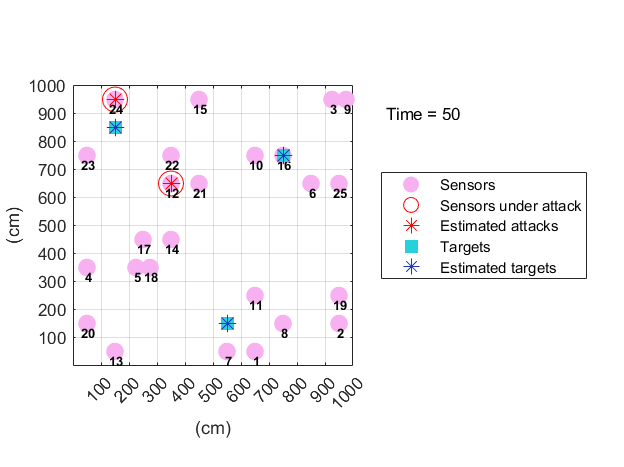
\includegraphics[scale=0.3]{img/aware_2a_3x_cs_1.png}}
    \caption{Aware: Three targets and two sensors under attack}
    \label{fig:aware_3}
\end{figure}

\begin{table}[h!]
\centering
\begin{tabular}{|c|c|c|c|}
\hline
\multirow{2}{*}{\textbf{For 100 iterations}} & \multicolumn{2}{|c|}{\textbf{attack $a$}} & \multicolumn{1}{|c|}{\textbf{state $x$}} \\
\cline{2-4}
 & \textbf{1-25} & \textbf{26-50} & \textbf{1-50} \\
\hline
\textbf{\% convergence} &99\% &76\% &80\% \\
\hline
\textbf{Mean time of convergene} &4.71 &45.73 &36.16 \\
\hline
\textbf{Minimum time of convergence} &2 &36 &12 \\
\hline
\textbf{Maximum time of convergence} &16 &50 &50 \\
\hline
\textbf{Temporay loss of tracking} &6\% &1\% &62\% \\
\hline
\end{tabular}
\caption{Summary table showing some statistics on $a$ and $x$}
\label{table:5}
\end{table}
    
    \subsubsection*{3\# optional task: Maximum number of sensors under attack}
    To determine the maximum number of sensors under attack, a convergence threshold of at least 50 percent was cosidered for both state x and attack a for both 100 simulation in a time period of 100. A maximum number of sensors under attack was found to be 7 with 5 targets to be tracked.
    \begin{figure}[h]   
        \vspace{-1cm}
        \centering 
        \subfigure[Convergence]
        {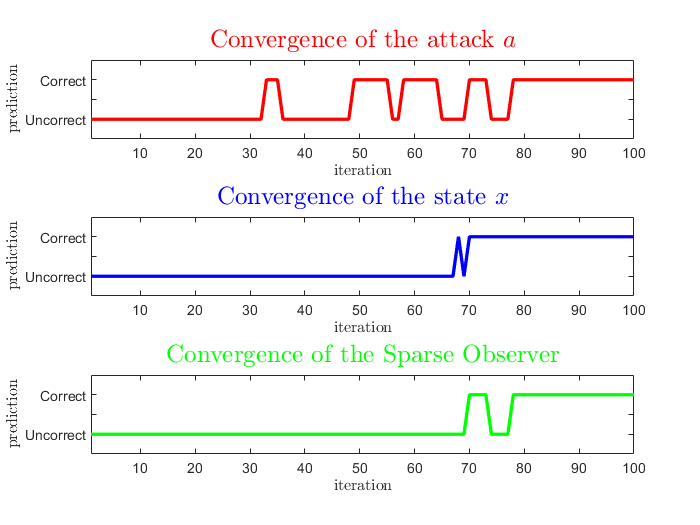
\includegraphics[scale=0.3]{img/aware_7a_5x_2.png}}
        \subfigure[Room]
        {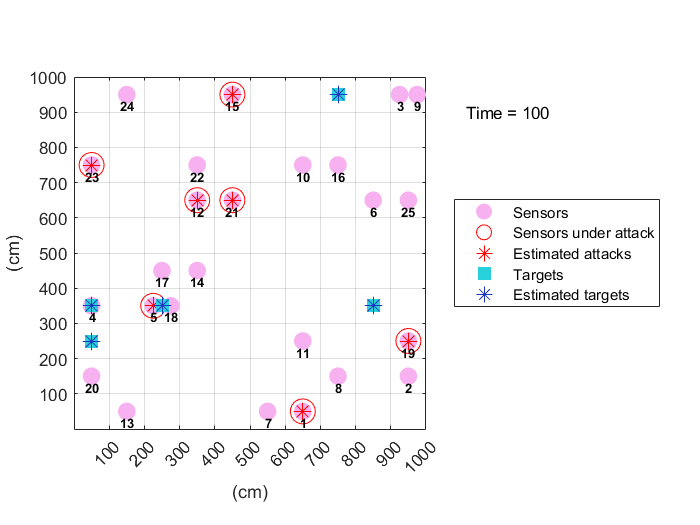
\includegraphics[scale=0.3]{img/aware_7a_5x_1.png}}
        \caption{Aware: Five targets and seven sensors under attack}
        \label{fig:aware_4}
    \end{figure}

\begin{table}[h!]
\centering
\begin{tabular}{|c|c|c|}
\hline
\multirow{2}{*}{\textbf{For 100 iterations}} & \multicolumn{1}{|c|}{\textbf{attack $a$}} & \multicolumn{1}{|c|}{\textbf{state $x$}} \\
\cline{2-3}
 & \textbf{1-100} & \textbf{1-100}\\
\hline
\textbf{\% convergence} &51\% &59\%  \\
\hline
\textbf{Mean time of convergene} &41.76 &71.64 \\
\hline
\textbf{Minimum time of convergence} &6 &27  \\
\hline
\textbf{Maximum time of convergence} &100 &99 \\
\hline
\textbf{Temporay loss of tracking} &32\% &37\%  \\
\hline
\end{tabular}
\caption{Summary table showing some statistics on $a$ and $x$}
\label{table:6}
\end{table}


    
    \subsection*{Additional comments}
    For data cleaning, we used prior information about the number of targets, whereas for the number of sensors under attack, we used a threshold. This is because, in reality, assuming knowledge of the number of sensors under attack is not plausible. Specifically, we assumed that if the estimated attack on a sensor was below 50\% of the highest recorded value at that moment for all sensors, then that value would be set to zero. Of course, this approach yields worse performance compared to filtering the data with knowledge of the number of sensors under attack, but it is also the most realistic.
